%  LaTeX support: latex@mdpi.com

%=================================================================
\documentclass[apajournal,article,submit,pdftex,moreauthors]{Definitions/mdpi}

%=================================================================
% MDPI internal commands - do not modify
\firstpage{1}
\makeatletter
\setcounter{page}{\@firstpage}
\makeatother
\pubvolume{1}
\issuenum{1}
\articlenumber{0}
\pubyear{2026}
\copyrightyear{2026}
\datereceived{ }
\daterevised{ }
\dateaccepted{ }
\datepublished{ }

%=================================================================
% Full title of the paper
\Title{GATrESN: An AI-Driven Digital Twin Framework for Strategic Operations Management}

% Author ORCID IDs
\newcommand{\orcidauthorA}{0000-0001-6077-6458}
\newcommand{\orcidauthorB}{0000-0002-3234-6589}

% Authors
\Author{Cesar H. Valencia $^{1,}$*\orcidA{} and Laura M. Valencia $^{2}$\orcidB{}}

% Authors for metadata in PDF
\AuthorNames{Cesar H. Valencia and Laura M. Valencia}

% Affiliations
\address{%
$^{1}$ \quad Universidad Santo Tom\'as, Bucaramanga, Colombia; cesar.valencia@ustabuca.edu.co\\
$^{2}$ \quad Universidade Federal do Rio de Janeiro, Rio de Janeiro, Brazil; laura.valencia@facc.ufrj.br}

% Corresponding author
\corres{Correspondence: cesar.valencia@ustabuca.edu.co}

% Abstract
\abstract{Strategic operations management requires decision-support systems capable of representing enterprise behavior, anticipating uncertainty, and evaluating strategic actions before implementation. Conventional planning approaches often separate forecasting, simulation, and optimization, which limits their ability to evaluate how capacity, cost, inventory, workforce, resilience, and supplier decisions interact under uncertain future conditions. This paper proposes GATrESN, an AI-driven digital twin framework that integrates Echo State Networks, Transformer-style attention, and Genetic Algorithms for predictive--prescriptive strategic operations management. The framework represents the organization as a dynamic digital twin whose virtual state includes demand, capacity, cost, service pressure, labor availability, inventory coverage, and operational risk. Unlike descriptive monitoring systems, the proposed digital twin acts as a scenario-based digital laboratory for decision experimentation: it reconstructs temporal operational states, forecasts future demand and risk, simulates uncertain operating conditions, evaluates candidate strategic policies, and feeds KPI information back into the virtual representation. The computational model links ESN-based nonlinear temporal memory, attention-based dependency weighting, Monte Carlo scenario generation, and GA-based robust policy search in a reproducible MATLAB workflow. The case study is organized as a longitudinal site--product--period panel with 24 operational sites, 16 product families, 640 planning periods, 245,760 operational records, 1800 matched strategic decision instances, and 35 Monte Carlo scenarios per decision. GATrESN is compared with a simplified linear programming policy and a rule-based managerial policy using the same digital twin states and performance indicators. Results show that GATrESN achieved the highest mean strategic score, improved service-level performance, and substantially reduced residual risk relative to both benchmarks, while explicitly exposing the cost--risk trade-off associated with resilience-oriented decisions. Paired statistical validation across matched decision states confirmed positive GATrESN advantages for strategic score, service level, and residual-risk reduction, with bootstrap confidence intervals above zero and large paired effect sizes. These findings demonstrate that an AI-driven digital twin can operate as a reproducible digital laboratory for robust, scenario-aware, and statistically validated strategic operations management.}

% Keywords
\keyword{GATrESN; digital twin; digital laboratory; artificial intelligence; echo state network; transformer attention; genetic algorithm; strategic operations management; simulation; decision support}

%%%%%%%%%%%%%%%%%%%%%%%%%%%%%%%%%%%%%%%%%%
\begin{document}

%%%%%%%%%%%%%%%%%%%%%%%%%%%%%%%%%%%%%%%%%%
\section{Introduction}
Organizations operate under increasing uncertainty, driven by demand variability, resource constraints, supply disruptions, technological change, and competitive pressure. Strategic operations management must therefore move beyond static planning models and adopt adaptive decision-support systems that connect operational data, predictive intelligence, and scenario-based evaluation. In distributed enterprises, strategic decisions such as capacity expansion, cost-policy adjustment, inventory buffering, workforce flexibility, and resilience investment are interdependent, dynamic, and exposed to uncertainty. A decision that appears efficient under nominal demand may become fragile when disruptions affect capacity, labor availability, service pressure, or supplier reliability. Consequently, strategic operations management requires computational frameworks capable of evaluating not only expected performance, but also robustness, risk exposure, and the operational consequences of alternative managerial actions before implementation.

Digital twin research has increasingly emphasized the integration of cyber-physical data, simulation, and decision support as a mechanism for monitoring and improving operational systems \citep{tao2019digital,fuller2020digital}. Digital twins provide a promising mechanism for representing real or conceptual systems in a dynamic computational environment. In manufacturing and supply chain contexts, prior research has distinguished digital models, digital shadows, and digital twins according to the degree of data integration and feedback between physical and virtual systems \citep{kritzinger2018digital}. This distinction is important for strategic operations management because a static model or dashboard can describe a system, but it cannot fully support adaptive strategic reasoning unless it can preserve system state, simulate future scenarios, evaluate decisions, and feed performance information back into the virtual representation.

When combined with artificial intelligence, digital twins can evolve from descriptive replicas into predictive and prescriptive decision-support platforms. In this context, an AI-driven digital twin can support strategic operations management by forecasting future states, simulating strategic alternatives, detecting performance deviations, and recommending adaptive actions. It can also operate as a digital laboratory in which strategic policies are tested virtually before resources are committed in the organization. However, the value of such a system depends on the explicit connection between the virtual state of the organization, the predictive model used to estimate future operating conditions, the scenario engine used to represent uncertainty, and the prescriptive mechanism used to select strategic policies. Treating these components separately may lead to fragmented decision support: forecasting models may be accurate but non-prescriptive, optimization models may be mathematically tractable but dynamically simplified, and simulation models may be informative but computationally disconnected from adaptive policy search.

This paper addresses this methodological gap by proposing GATrESN, an AI-driven digital twin framework for strategic operations management. The framework combines Echo State Networks (ESNs) for temporal operational memory, Transformer-style attention for long-range dependency extraction, and Genetic Algorithms (GAs) for strategic decision optimization. This hybrid design is motivated by the ability of reservoir computing to model nonlinear temporal systems with efficient readout training \citep{jaeger2004harnessing,lukosevicius2009reservoir}, the ability of attention mechanisms to weight relevant sequence elements \citep{bahdanau2014neural,vaswani2017attention}, and the suitability of evolutionary search for multi-criteria optimization problems \citep{deb2002fast}. Rather than presenting these techniques as independent modules, GATrESN embeds them in a single digital twin loop: operational states are encoded through reservoir dynamics, temporally relevant dependencies are emphasized through attention, future operating conditions are forecasted, uncertain scenarios are simulated, and strategic decisions are optimized according to service, utilization, cost, and residual-risk objectives.

The central contribution is therefore the digital twin logic that connects a virtual operational state, AI-based state forecasting, scenario simulation, prescriptive policy search, and KPI feedback into one reproducible decision-support loop. The contribution is threefold: first, it presents a modular architecture connecting organizational data, digital twin state representation, AI analytics, scenario simulation, and strategic decision support; second, it integrates ESNs, Transformer-style attention, and GAs into a reproducible digital twin decision model; third, it demonstrates the framework through a simulation-based case study implemented in MATLAB. By emphasizing reproducibility, explicit mathematical formulation, benchmark comparison, and the digital-laboratory role of the twin, the study aims to provide a rigorous foundation for AI-driven digital twins as strategic operations management tools rather than as purely descriptive monitoring systems.

The remainder of the paper is organized as follows. Section~2 reviews the literature on digital twins, artificial intelligence, and strategic decision support. Section~3 presents the proposed GATrESN digital twin framework, including the strategic operations problem, operational data structure, digital twin representation, architecture, and computational model. Section~4 reports the experimental results, benchmark comparisons, and paired statistical validation. Sections~5 and~6 discuss the implications of the findings and conclude the paper, respectively.

%%%%%%%%%%%%%%%%%%%%%%%%%%%%%%%%%%%%%%%%%%
\section{Literature Background}
\subsection{Digital Twins in Operations Management}
Digital twins have been widely discussed as virtual representations of physical or organizational systems. In operations management, they enable monitoring, simulation, and decision support across production, logistics, maintenance, and service systems \citep{tao2018digital,tao2019digital,fuller2020digital,zheng2022smart,singh2023review}. Digital twin-driven manufacturing research highlights the convergence of physical product data, virtual models, and lifecycle information as a basis for improving design, manufacturing, and service processes \citep{tao2018digital,kusiak2018smart,uhlemann2019digital,zhang2020knowledge}. Similarly, the relationship between digital twins, big data, and Industry 4.0 has been described as a key pathway for transforming manufacturing systems from isolated automation toward connected and data-intensive operational intelligence \citep{qi2018digital,tortorella2021industry,holmstrom2020digital}.

The digital twin concept is particularly relevant for operations management because it provides a structured way to connect state representation, system behavior, and decision feedback. A digital twin is not only a visualization layer; it can operate as a computational environment in which alternative actions are evaluated before being transferred to the real organization. The distinction between digital models, digital shadows, and digital twins is therefore central: a digital model may represent an asset or process, a digital shadow may update through operational data, but a digital twin implies a stronger bidirectional relationship between the system and its virtual counterpart \citep{kritzinger2018digital}. For strategic operations management, this distinction implies that the virtual representation should support scenario experimentation, policy testing, and performance feedback rather than only reporting historical indicators.

In supply chains and distributed operations, digital twins have been proposed as mechanisms for improving resilience, managing disruption risk, stress-testing operational networks, and supporting decisions under uncertainty. The digital supply chain twin, for example, has been framed as a tool for disruption-risk management and resilience analysis in Industry 4.0 contexts \citep{ivanov2021digital,ivanov2019ripple,burgos2021food,ivanov2023idt,nascimento2022cloud}. Digital twins have also been used for scheduling and resource-allocation problems in manufacturing systems \citep{fang2019jobshop,zhang2021dynamic,leng2021automated,liu2021shared,zhang2024schedulingreview}. This perspective is consistent with the strategic operations problem addressed in this paper, where managerial actions must balance efficiency, service continuity, capacity utilization, and residual risk. Nevertheless, many digital twin studies remain concentrated on architecture, lifecycle integration, and operational monitoring, while the explicit integration of predictive learning and prescriptive optimization into the twin remains an open methodological challenge.

\subsection{Artificial Intelligence for Strategic Decision Support}
Artificial intelligence techniques, including machine learning, forecasting, anomaly detection, and optimization, can enhance strategic decisions by identifying patterns and estimating future system behavior. In operations management, AI becomes especially relevant when decisions depend on temporal dependencies, nonlinear interactions, and uncertain future states \citep{toorajipour2021ai,boonmee2019prescriptive,bertsimas2024explainable}. Strategic operations problems often involve time-dependent demand, capacity restrictions, cost variation, labor availability, inventory coverage, and operational-risk exposure. These variables interact dynamically, which makes purely static planning models insufficient for adaptive decision support.

ESNs and reservoir computing are particularly relevant for temporal operational data because the recurrent reservoir maps input histories into a nonlinear state space while only the readout layer is trained \citep{jaeger2004harnessing,lukosevicius2009reservoir,salinas2024esnreview}. Reservoir computing is rooted in the broader idea that complex recurrent dynamics can be exploited for real-time computation without requiring full recurrent-network training \citep{maass2002realtime,nakajima2022reservoir}. This property is attractive for strategic operations contexts where reproducibility, computational efficiency, and interpretable simulation workflows are important. Because the reservoir can be generated with fixed random seeds and controlled spectral properties, ESN-based models can provide a practical compromise between nonlinear temporal representation and reproducible experimentation.

Attention mechanisms provide an additional layer of temporal selectivity. Early attention-based sequence models allowed neural systems to focus on relevant input segments \citep{bahdanau2014neural}, while the Transformer architecture demonstrated that self-attention can represent sequence dependencies without relying entirely on recurrence \citep{vaswani2017attention}. Recent time-series research has extended Transformer-based models to long-sequence and multi-horizon forecasting problems \citep{zhou2021informer,lim2021tft,wen2026transformersurvey}. For an operations digital twin, attention can be used not as a black-box replacement for simulation, but as a mechanism to emphasize the historical states most relevant to current demand, risk, utilization, and capacity decisions.

Finally, evolutionary optimization is suitable when strategic decision variables must be selected under nonlinear trade-offs. Genetic algorithms and elitist evolutionary search have been widely used for complex multi-objective optimization where analytical gradients may be unavailable or insufficient \citep{deb2002fast}. Robust and data-driven optimization studies in supply chain planning further emphasize the importance of evaluating decisions under uncertainty rather than optimizing only nominal operating conditions \citep{gao2019robust,ning2021datadriven,basciftci2022vaccine,perea2022feedback,ghasemian2025resilient}. This makes GA-based search appropriate for optimizing capacity adjustment, cost policy, resilience investment, inventory buffering, workforce flexibility, and supplier redundancy within a digital twin. In a strategic operations context, the relevant objective is rarely a single cost-minimization criterion; instead, decision-makers must consider service level, utilization, expected cost, and risk simultaneously. Evolutionary search is therefore useful because it can explore nonconvex policy spaces and evaluate candidate strategies through simulation-based objective functions.

The integration of temporal learning, attention, and evolutionary optimization is particularly promising for AI-driven digital twins. Temporal models estimate the evolving state of the system, attention mechanisms identify which portions of the operational history are most informative, and evolutionary search evaluates alternative strategic actions under simulated uncertainty. When embedded inside a digital twin, these components can transform the twin from a passive representation into an active predictive--prescriptive environment.

\subsection{Research Gap}
Although digital twins and AI have been studied in operational contexts, there remains a need for integrated frameworks that explicitly connect AI-driven digital twins with strategic operations management. Existing studies often emphasize digital twin architecture, lifecycle data integration, or operational monitoring, while fewer approaches integrate temporal learning, attention-based dependency extraction, and evolutionary optimization into a single reproducible strategic decision workflow. This gap is important because strategic operations decisions require more than accurate prediction: they require the ability to evaluate alternative actions under uncertainty and to translate predicted states into robust managerial policies.

Three limitations can be identified in the current literature. First, many digital twin studies focus on representation and monitoring rather than on prescriptive strategic decision-making. Second, many AI applications emphasize forecasting performance but do not embed the forecast inside a closed-loop decision environment. Third, optimization models often simplify the temporal and nonlinear structure of operations in order to maintain analytical tractability. The proposed GATrESN framework addresses these limitations by linking digital twin state representation, ESN-based temporal encoding, attention-based dependency weighting, Monte Carlo scenario simulation, GA-based policy search, and KPI feedback in a single reproducible workflow. In particular, the literature requires models that link predictive analytics, scenario simulation, and multi-criteria strategic evaluation while preserving the digital twin as the central organizing mechanism of the decision-support system.

%%%%%%%%%%%%%%%%%%%%%%%%%%%%%%%%%%%%%%%%%%
\section{Proposed GATrESN Digital Twin Framework}
\subsection{Strategic Operations Problem and Case Study Context}
The strategic operations problem addressed in this study concerns the management of a distributed enterprise network in which multiple operational sites and product families must be coordinated under uncertain demand, heterogeneous capacity, variable cost structures, service-level pressure, and operational risk. In this environment, managerial decisions are not limited to forecasting future demand or selecting a single production quantity; rather, they involve the simultaneous selection of capacity-adjustment policies, cost-control actions, resilience investments, inventory buffers, workforce-flexibility actions, and supplier-redundancy levels whose effects propagate over time and interact with the current state of the organization. A capacity expansion may improve service reliability but increase operating cost; an aggressive cost policy may improve short-term efficiency but reduce service quality and flexibility under disruption; excessive inventory or redundancy may reduce residual risk but introduce additional operating cost; and insufficient resilience investment may leave the system vulnerable to demand shocks, labor constraints, inventory shortages, or site-specific risk events.

The case study represents a Strategic Operations Network responsible for delivering several product families under uncertain demand and resource conditions. The organization is structured as an enterprise-scale operating system with 24 operational sites, 16 product families, and 640 sequential planning periods, producing more than 245,000 operational records before supervised lag transformation. Each site is interpreted as a semi-autonomous operational unit with its own capacity profile, cost structure, labor availability, inventory coverage, and exposure to operational risk. Each product family introduces differentiated demand patterns, volatility, and service pressure. The operational context is intentionally defined at the strategic-tactical interface: the objective is not to reproduce a single shop-floor process, but to evaluate how an AI-driven digital twin can support managerial decisions that affect capacity allocation, cost policy, service reliability, inventory buffering, workforce flexibility, supplier redundancy, and resilience investment across a distributed organization.

Let $\mathcal{I}=\{1,\ldots,N_s\}$ denote the set of operational sites, $\mathcal{P}=\{1,\ldots,N_p\}$ the set of product families, and $\mathcal{T}=\{1,\ldots,N_t\}$ the set of planning periods. For each site--product--period tuple $(i,p,t)$, the operational state is represented by:

\begin{linenomath}
\begin{equation}
\mathbf{x}_{i,p,t}
=
\left[
D_{i,p,t},
C_{i,p,t},
c_{i,p,t},
\psi_{i,p,t},
\rho_{i,p,t},
\ell_{i,t},
v_{i,p,t}
\right]^{\top},
\label{eq:operations_state}
\end{equation}
\end{linenomath}
where $D_{i,p,t}$ is demand, $C_{i,p,t}$ is base capacity, $c_{i,p,t}$ is unit cost, $\psi_{i,p,t}=D_{i,p,t}/C_{i,p,t}$ is service pressure, $\rho_{i,p,t}$ is external operational risk, $\ell_{i,t}$ is labor availability, and $v_{i,p,t}$ is inventory coverage. The strategic decision vector for a decision instance at time $t$ is:

\begin{linenomath}
\begin{equation}
\mathbf{z}_{t}
=
\left[
m^C_t,\,
m^K_t,\,
r_t,\,
b_t,\,
f_t,\,
q_t
\right]^{\top}
\in \Omega_z,
\label{eq:strategic_problem_decision}
\end{equation}
\end{linenomath}
where $m^C_t$ is the capacity multiplier, $m^K_t$ is the cost-policy multiplier, $r_t$ is resilience investment, $b_t$ is the inventory-buffer level, $f_t$ is workforce flexibility, $q_t$ is supplier redundancy, and $\Omega_z$ denotes the bounded feasible policy space. The strategic operations problem can be stated as the robust policy-selection problem:

\begin{linenomath}
\begin{equation}
\max_{\mathbf{z}_t\in\Omega_z}
\;
\mathcal{J}_{t}(\mathbf{z}_t)
=
\mathbb{E}_{\omega\in\Omega}
\left[
J_t^{\omega}(\mathbf{z}_t \mid \widehat{\mathbf{x}}_{t+1}^{\omega})
\right]
-
\lambda_R
\operatorname{Risk}_{\omega}
\left[
J_t^{\omega}(\mathbf{z}_t \mid \widehat{\mathbf{x}}_{t+1}^{\omega})
\right],
\label{eq:strategic_problem_objective}
\end{equation}
\end{linenomath}
subject to:

\begin{linenomath}
\begin{align}
S_t^{\omega}(\mathbf{z}_t) &\geq S_{\min}, &
0 \leq R_t^{\omega}(\mathbf{z}_t) &\leq R_{\max}, \label{eq:strategic_constraints_a}\\
U_{\min} \leq U_t^{\omega}(\mathbf{z}_t) &\leq U_{\max}, &
K_t^{\omega}(\mathbf{z}_t) &\leq K_{\max}, \quad \forall \omega\in\Omega,
\label{eq:strategic_constraints_b}
\end{align}
\end{linenomath}
where $J_t^{\omega}$ is the scenario-level strategic utility, $\widehat{\mathbf{x}}_{t+1}^{\omega}$ is a possible future operational state generated inside the digital twin, $S_t^{\omega}$ is service level, $U_t^{\omega}$ is utilization, $K_t^{\omega}$ is expected cost, and $R_t^{\omega}$ is residual risk. Equations~\eqref{eq:strategic_problem_objective}--\eqref{eq:strategic_constraints_b} formalize the engineering problem: the model must identify a decision vector that performs well not only for a single predicted future, but across a family of plausible operating scenarios before managerial action is implemented.

\begin{figure}[H]
\centering
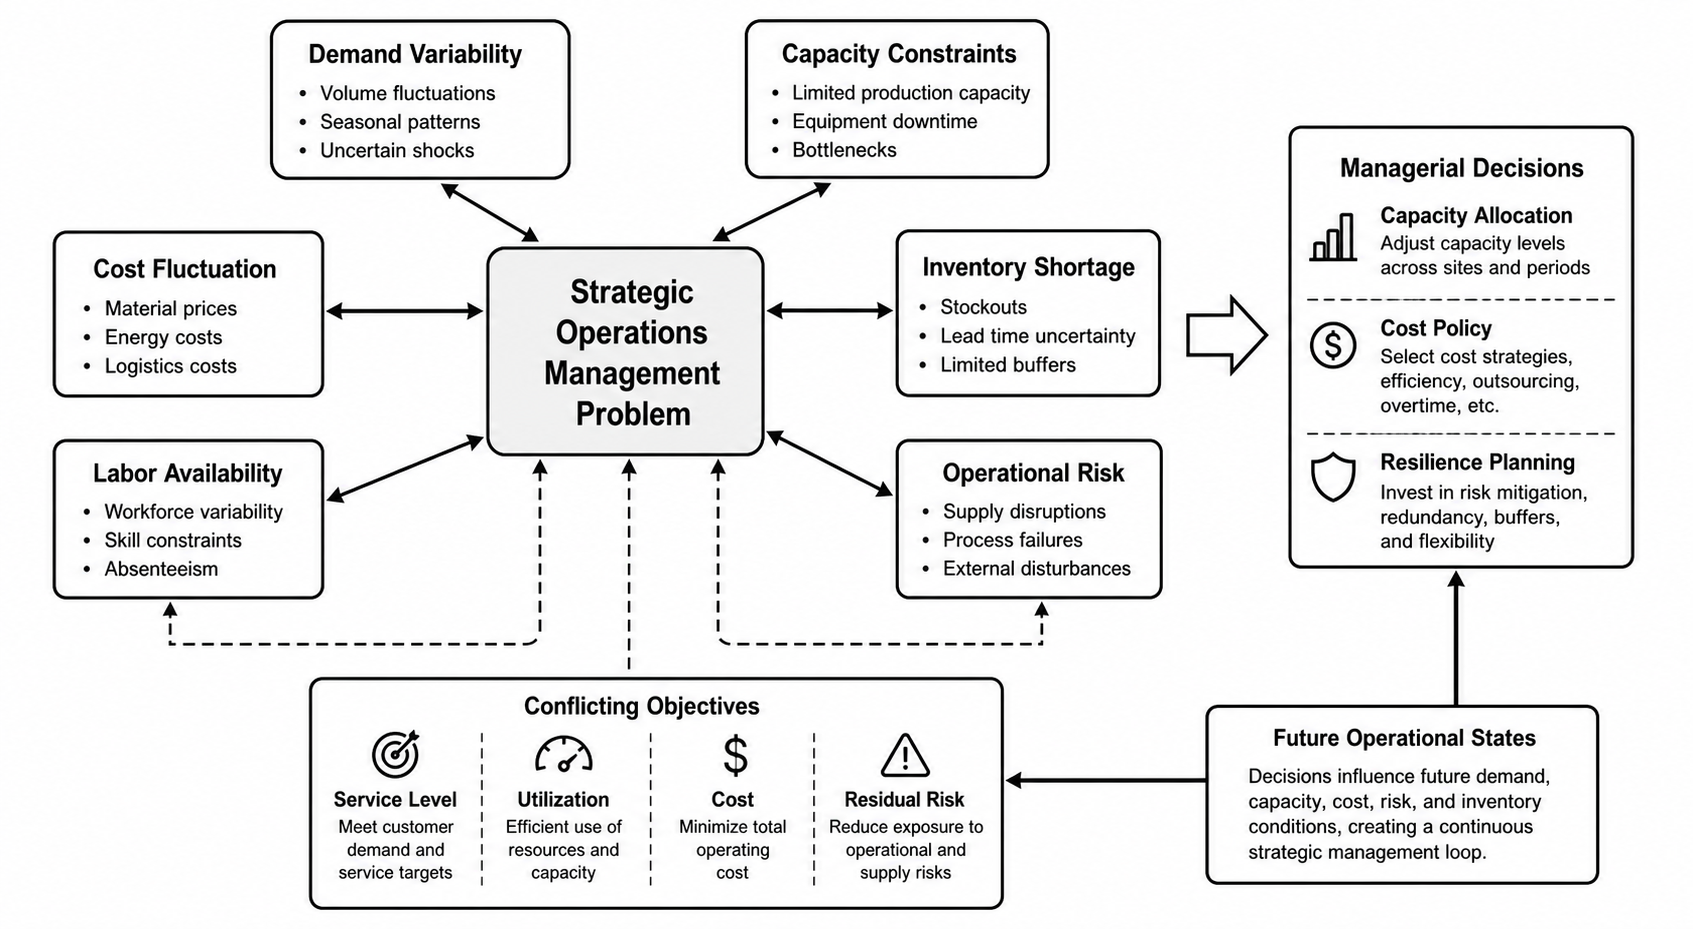
\includegraphics[width=0.98\textwidth]{../figures/GATrESN_problem_context_ai.png}
\caption{Strategic operations management problem under uncertainty, showing interacting demand, capacity, cost, labor, inventory, and operational-risk pressures that must be balanced through managerial decisions.\label{fig:strategic_operations_problem}}
\end{figure}

\subsection{Operational Data Structure}
The operational data are organized as a longitudinal site--product--period panel. Each record corresponds to one tuple $(i,p,t)$, where $i$ identifies the operational site, $p$ identifies the product family, and $t$ identifies the sequential planning period. The main experimental configuration contains 24 operational sites, 16 product families, and 640 planning periods, resulting in 245,760 operational records before lag construction. This structure is sufficiently broad to represent spatial heterogeneity across sites, product-specific demand behavior, and temporal dependencies across planning periods.

The dataset contains 10 variables. Three variables define the panel index: \textit{Site}, \textit{Product}, and \textit{Period}. Site and Product are categorical identifiers encoded as integers, whereas Period is an ordered temporal index. The remaining seven variables are continuous numerical operational indicators: demand, base capacity, unit cost, service pressure, external risk, labor availability, and inventory coverage. Demand represents the requested operating load; base capacity represents available operating capability before strategic adjustment; unit cost captures the operating-cost level; service pressure measures the relationship between demand and capacity; external risk captures disruption exposure; labor availability measures workforce readiness; and inventory coverage represents buffer availability. No missing values are present in the generated computational dataset used by the model pipeline.

\begin{figure}[H]
\centering
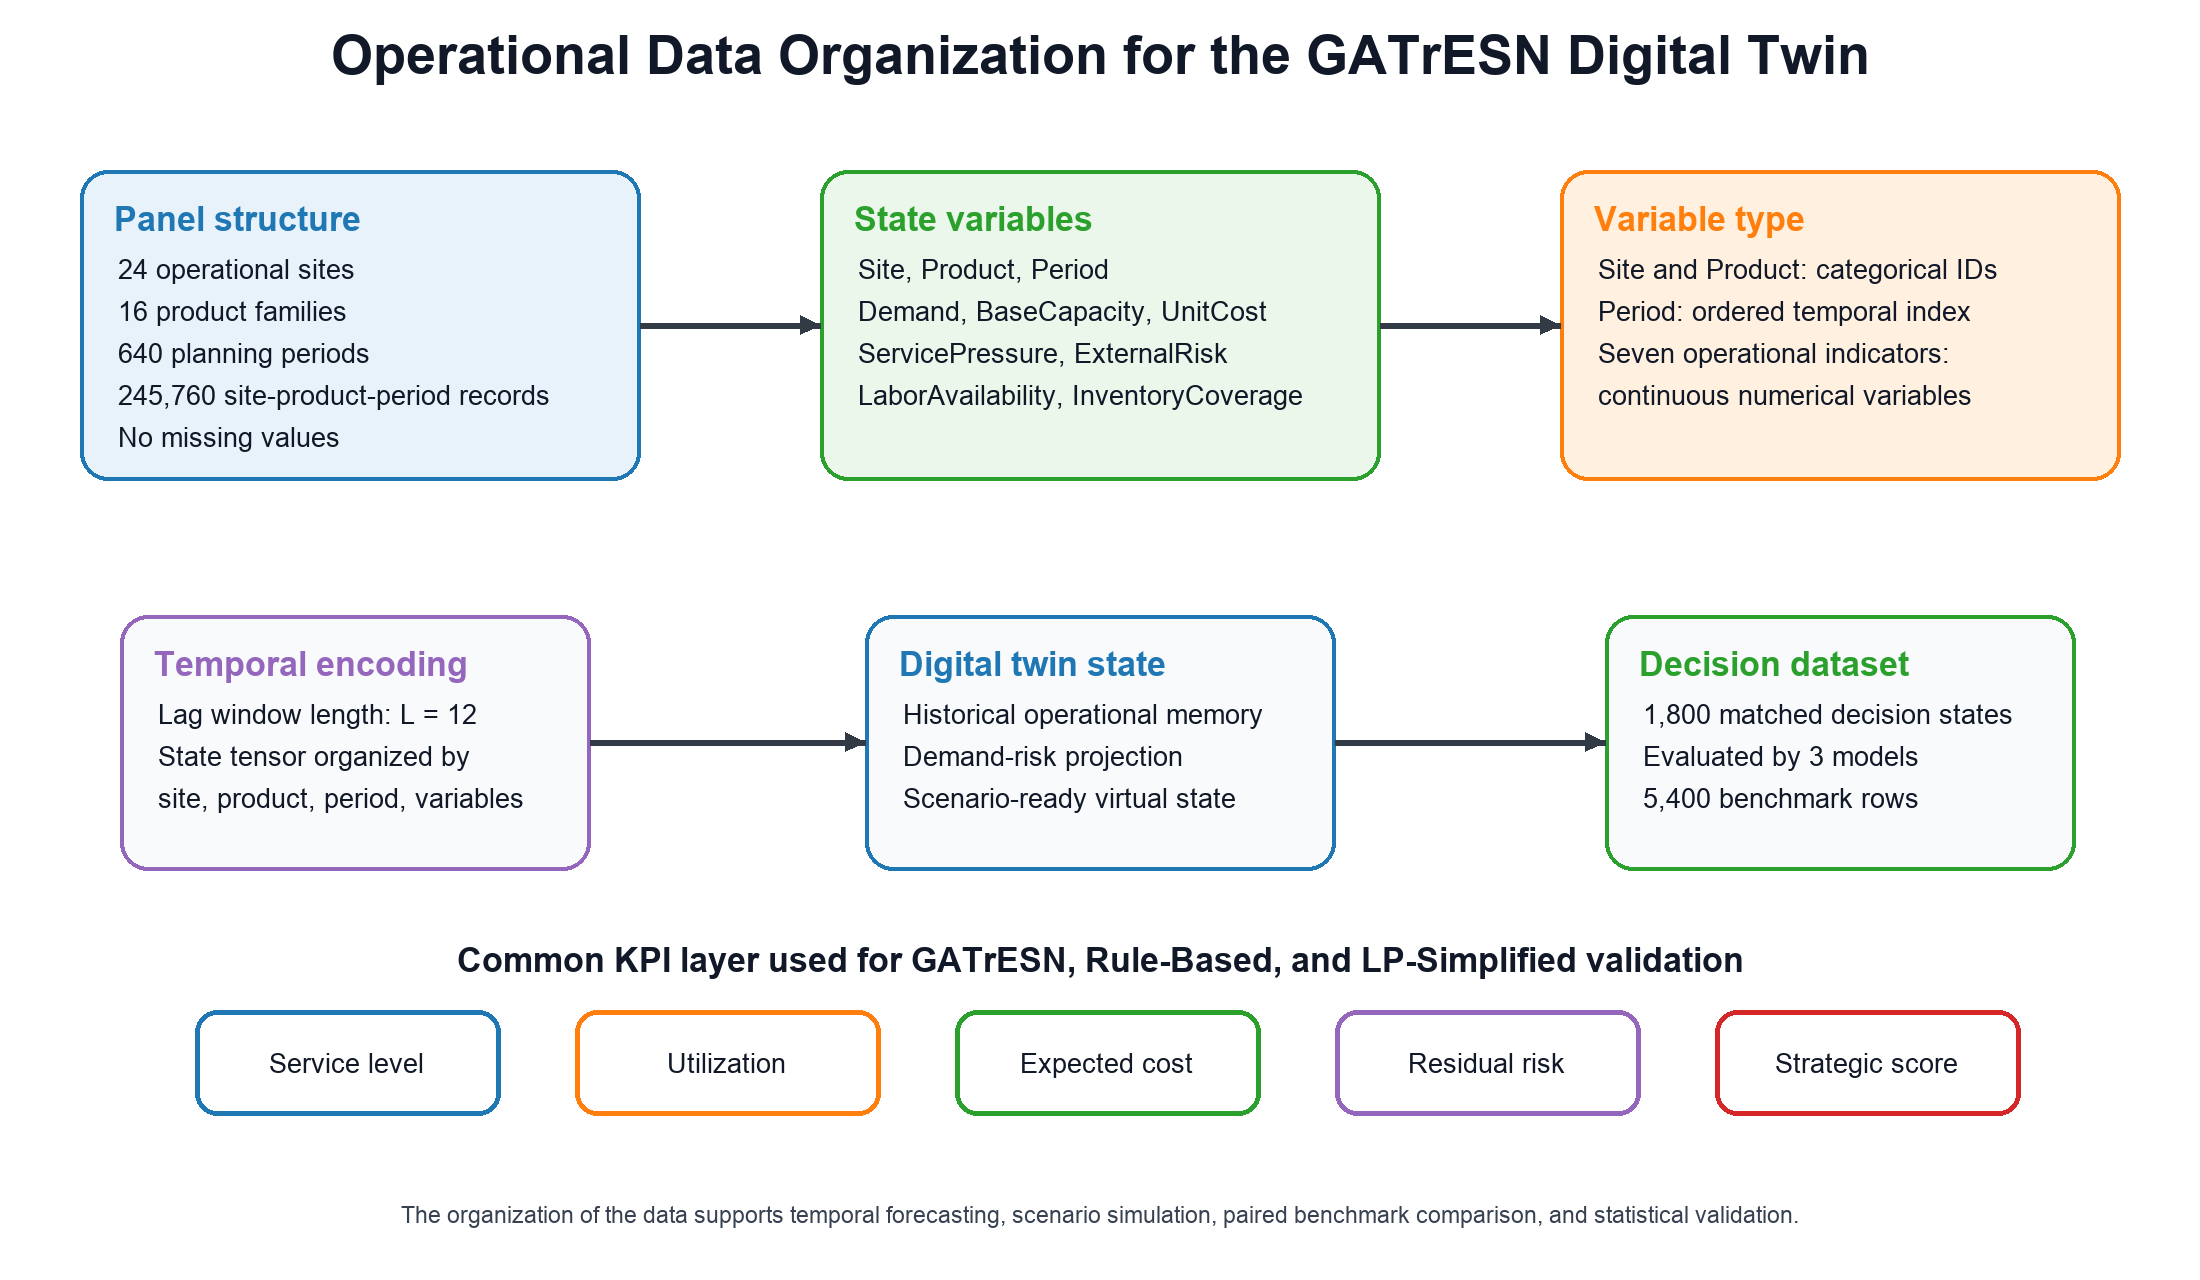
\includegraphics[width=0.98\textwidth]{../figures/GATrESN_data_organization.png}
\caption{Organization of the operational data used by the GATrESN digital twin, from the site--product--period panel to lagged temporal states, matched decision instances, benchmark comparison, and KPI-based validation.\label{fig:data_organization}}
\end{figure}

Figure~\ref{fig:data_organization} shows how the operational data are transformed into digital twin states. The raw panel is first ordered by site, product, and period. The seven continuous indicators are then converted into lagged temporal windows of length $L=12$, allowing the ESN--attention layer to learn from recent operational history rather than from isolated observations. These lagged states feed the digital twin representation, where future demand and risk are forecasted and scenario-ready virtual states are created. The prescriptive stage evaluates 1800 matched decision states, each of which is solved by GATrESN and re-evaluated under the Rule-Based and LP-Simplified benchmark policies. As a result, the benchmark dataset contains 5400 rows, corresponding to the same 1800 decision states evaluated by three decision mechanisms.

\begin{table}[H]
\caption{Operational data structure used by the digital twin.\label{tab:data_structure}}
\begin{tabularx}{\textwidth}{CCCC}
\toprule
\textbf{Component} & \textbf{Role} & \textbf{Type} & \textbf{Scale}\\
\midrule
Site & Operational unit identifier & Categorical ID & 24 levels\\
Product & Product-family identifier & Categorical ID & 16 levels\\
Period & Sequential planning index & Ordered temporal index & 640 periods\\
Demand & Operating load & Continuous numerical & 17.17--214.38\\
Base capacity & Available capability & Continuous numerical & 64.41--137.31\\
Unit cost & Operating-cost level & Continuous numerical & 34.78--100.73\\
Service pressure & Demand-capacity pressure & Continuous numerical & 0.18--2.43\\
External risk & Disruption exposure & Continuous numerical & 0.00--1.00\\
Labor availability & Workforce readiness & Continuous numerical & 0.40--1.00\\
Inventory coverage & Buffer availability & Continuous numerical & 0.15--1.25\\
\bottomrule
\end{tabularx}
\end{table}

This organization is important for the proposed AI-driven digital twin because it preserves the three dimensions required by the strategic operations problem: cross-site heterogeneity, product-family heterogeneity, and temporal evolution. It also supports paired model validation because all decision mechanisms are evaluated on the same digital twin states and the same KPI definitions. Therefore, differences among GATrESN, Rule-Based, and LP-Simplified policies are attributable to the prescriptive decision logic rather than to changes in data structure, state representation, or evaluation criteria.

\subsection{Digital Twin Representation}
In this study, the digital twin is defined as a dynamic virtual representation of the strategic operations network rather than as a static dataset, dashboard, or standalone forecasting model. The twin maintains a time-indexed state vector describing the relevant operating condition of the enterprise, including demand, capacity, unit cost, service pressure, labor availability, inventory coverage, and operational risk. This state representation is updated through operational observations and transformed into lagged temporal windows so that the virtual system preserves memory of prior conditions, disruption persistence, and cross-period dependencies. The digital twin layer therefore acts as the computational environment in which the organization can be observed, projected, stressed, and evaluated before managerial action is implemented.

The central idea is that the digital twin represents possible solutions before they occur in the real system. A candidate strategy is not adopted directly; it is first injected into the virtual enterprise, exposed to uncertain scenarios, and evaluated through the same performance logic used to assess real operations. In this sense, the twin is a digital laboratory for strategic decision-making: it creates plausible futures, tests the consequences of strategic actions, and helps decision-makers understand what may happen if the organization increases capacity, reduces cost, invests in resilience, expands inventory buffers, improves workforce flexibility, or adds supplier redundancy. The digital twin therefore supports anticipatory management because it turns future uncertainty into simulated evidence before the organization commits resources.

The proposed digital twin performs five functions. First, it represents the current and historical operational state of the enterprise at site, product, and period levels. Second, it preserves temporal memory by converting operational observations into lagged windows. Third, it predicts future operating states through the ESN--attention forecasting core. Fourth, it creates scenario-based replicas of uncertain future conditions by applying demand, capacity, cost, and risk shocks to the predicted state. Fifth, it evaluates strategic policy alternatives by computing service level, utilization, expected cost, residual risk, and composite strategic score. The feedback layer closes the digital twin loop by returning KPI information to the virtual state representation, enabling the system to support adaptive strategic learning rather than one-shot optimization.

Mathematically, the digital twin at time $t$ is represented as:

\begin{linenomath}
\begin{equation}
\mathcal{T}_t
=
\left\{
\mathbf{x}_{t-L+1:t},
\boldsymbol{\theta}_{op},
\boldsymbol{\kappa}_{t},
\mathcal{M}_{AI},
\mathcal{S}_{MC}
\right\},
\label{eq:digital_twin_state}
\end{equation}
\end{linenomath}
where $\mathbf{x}_{t-L+1:t}$ is the observed operational history, $\boldsymbol{\theta}_{op}$ contains structural operating parameters such as site and product characteristics, $\boldsymbol{\kappa}_{t}$ contains KPI feedback from prior evaluations, $\mathcal{M}_{AI}$ denotes the embedded GATrESN predictive--prescriptive model, and $\mathcal{S}_{MC}$ denotes the scenario-generation mechanism. The twin evaluates a candidate policy through:

\begin{linenomath}
\begin{equation}
\left(
\widehat{\mathbf{x}}_{t+1}^{\omega},
\mathbf{k}_{t+1}^{\omega}
\right)
=
\mathcal{T}_t
\left(
\mathbf{z}_t,\omega
\right),
\quad
\omega\in\Omega,
\label{eq:twin_policy_evaluation}
\end{equation}
\end{linenomath}
meaning that each policy $\mathbf{z}_t$ is evaluated over a set of possible future scenarios before it is recommended.

\subsection{GATrESN Framework Architecture}
The proposed GATrESN framework is the operational structure that makes the digital twin predictive and prescriptive. It consists of six connected layers: the organizational system layer, the data layer, the digital twin state layer, the AI analytics layer, the strategic decision layer, and the feedback layer. These layers connect operational indicators, temporal forecasting, scenario simulation, strategic optimization, and KPI-based learning. The framework is aligned with the view that digital twins should support a structured connection between physical or organizational states, virtual representations, data analytics, and decision feedback \citep{kritzinger2018digital,fuller2020digital}.

\begin{figure}[H]
\centering
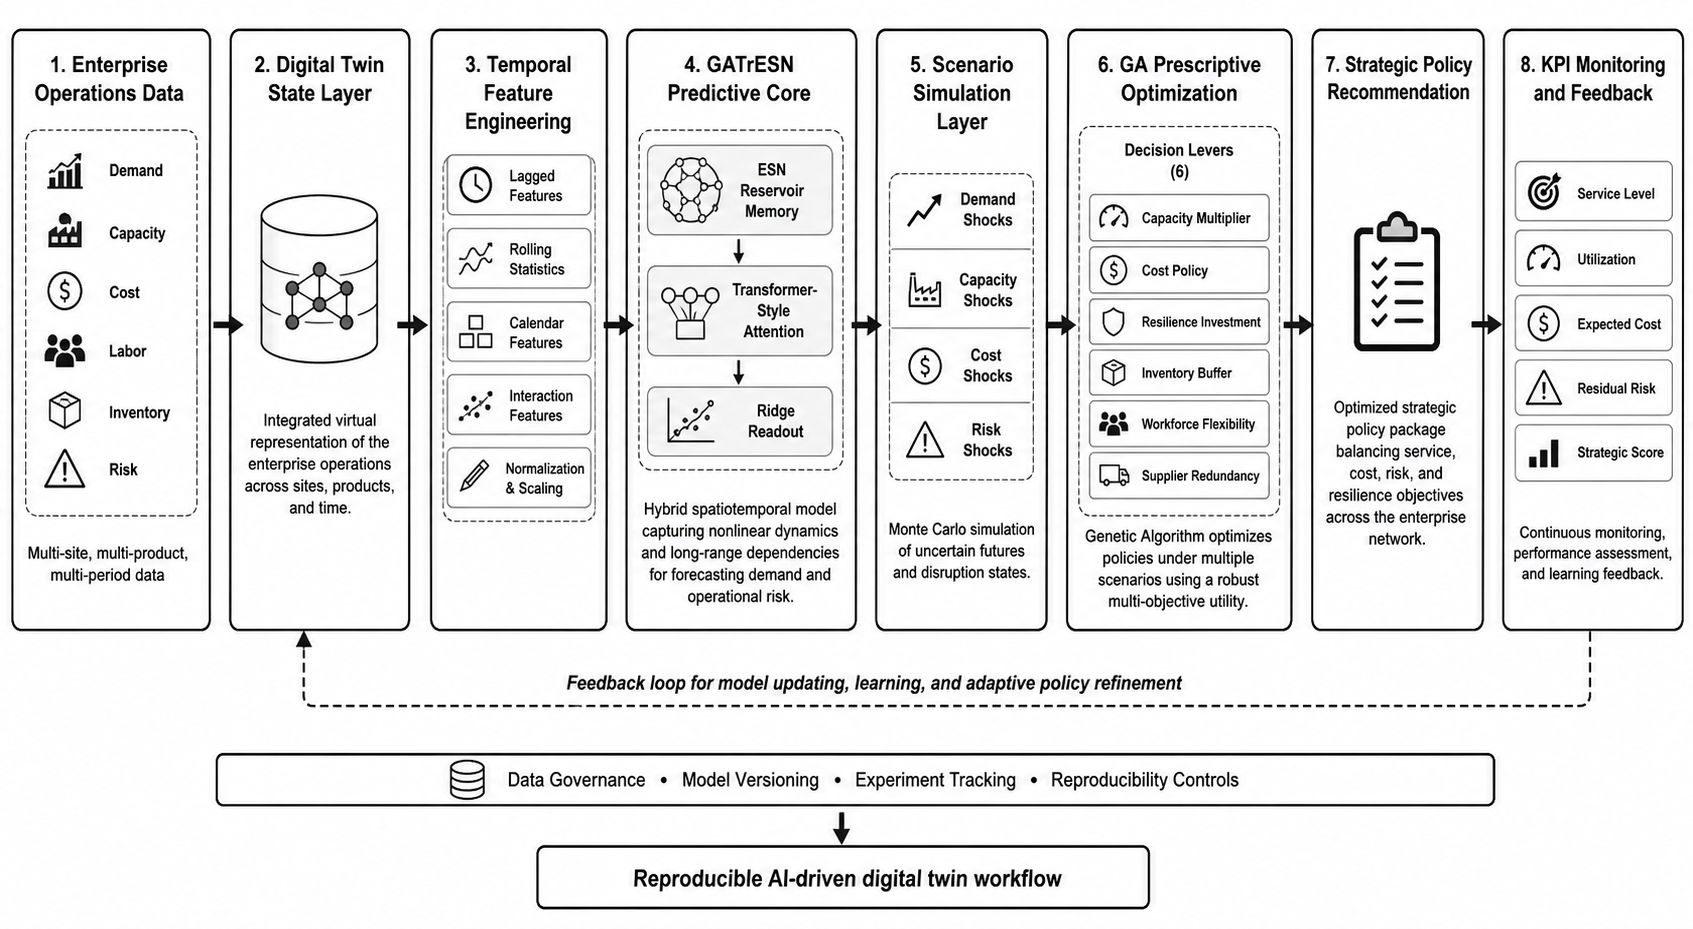
\includegraphics[width=0.98\textwidth]{../figures/GATrESN_model_architecture_ai.png}
\caption{Detailed architecture of the proposed GATrESN AI-driven digital twin framework, integrating enterprise operations data, digital twin state representation, temporal feature engineering, ESN--attention forecasting, scenario simulation, GA-based prescriptive optimization, and KPI feedback.\label{fig:gatr_esn_architecture}}
\end{figure}

The organizational system layer defines the real or conceptual strategic operations network: sites, product families, planning periods, capacity structures, cost profiles, labor availability, inventory coverage, and risk exposure. The data layer transforms these indicators into structured temporal windows. The digital twin state layer stores the operational memory of the system and provides the virtual environment in which future states are projected. The AI analytics layer contains the ESN--attention predictive core, which estimates future demand and risk from temporal operational patterns. The strategic decision layer uses the predicted state as input to a GA-based optimizer that searches over policy packages. Finally, the feedback layer returns service, utilization, cost, risk, and strategic-score indicators to the digital twin state, closing the loop between virtual experimentation and adaptive strategic learning.

This architecture is intentionally hybrid. The ESN is used because strategic operations data are temporal and nonlinear; attention is used because not all historical states are equally relevant to the next strategic decision; and the GA is used because the decision space is nonlinear, bounded, multi-criteria, and difficult to solve through a single closed-form optimization model. The result is not simply a combination of three algorithms, but a digital twin workflow in which temporal learning, scenario generation, and policy optimization are coupled around the same virtual representation of the enterprise.

\subsection{GATrESN Computational Model}
The GATrESN computational model is the core methodological contribution of this paper. It defines how the AI-driven digital twin converts an observed operational history into a recommended strategic policy. The model is built as a predictive--prescriptive chain. First, the ESN maps lagged operational states into nonlinear reservoir trajectories that preserve temporal memory. Second, Transformer-style attention assigns relevance weights to the reservoir trajectory so that the model can emphasize the historical states that matter most for the current decision. Third, a ridge readout converts the ESN--attention representation into forecasts of future demand and risk. Fourth, the digital twin generates possible future scenarios around those forecasts. Fifth, the GA searches for the strategic decision vector that maximizes robust utility across those scenarios.

GATrESN combines three computational components inside the digital twin. First, an ESN encodes nonlinear temporal dynamics through reservoir states. ESNs are a form of reservoir computing in which a fixed recurrent reservoir transforms input sequences into high-dimensional dynamic states, while a comparatively simple readout is trained for prediction \citep{jaeger2004harnessing,lukosevicius2009reservoir}. Second, a Transformer-style attention mechanism extracts long-range dependencies from lagged reservoir representations, following the broader principle that attention mechanisms can weight sequence elements according to their relevance \citep{bahdanau2014neural,vaswani2017attention}. Third, a GA optimizes strategic decision variables within the digital twin, including capacity adjustment, cost policy, resilience investment, inventory buffering, workforce flexibility, and supplier redundancy, following the use of evolutionary search for complex nonlinear optimization problems \citep{deb2002fast}. The AI components therefore operate as the predictive and prescriptive engines of the twin, while the digital twin provides the stateful environment in which forecasts, scenarios, decisions, and feedback are consistently evaluated.

The mathematical foundation of GATrESN is defined as a sequential predictive--prescriptive mapping that links digital twin state representation, reservoir-based temporal encoding, attention-based dependency weighting, scenario simulation, and evolutionary policy optimization. Let $\mathbf{x}_t \in \mathbb{R}^{d}$ denote the aggregated operational state vector of the digital twin at time $t$. For a lag length $L$, the digital twin observes the temporal window $\mathbf{X}_t=[\mathbf{x}_{t-L+1},\ldots,\mathbf{x}_{t}]$. The ESN component maps this window into nonlinear reservoir states according to:

\begin{linenomath}
\begin{equation}
\mathbf{h}_{\tau}
=
(1-\alpha)\mathbf{h}_{\tau-1}
+
\alpha \tanh \left(
\mathbf{W}_{in}\mathbf{x}_{\tau}
+
\mathbf{W}_{r}\mathbf{h}_{\tau-1}
\right),
\quad
\tau=t-L+1,\ldots,t,
\label{eq:esn_state}
\end{equation}
\end{linenomath}
where $\mathbf{h}_{\tau}\in \mathbb{R}^{n_r}$ is the reservoir state, $\alpha$ is the leak rate, $\mathbf{W}_{in}$ is the input matrix, and $\mathbf{W}_{r}$ is the recurrent reservoir matrix scaled to satisfy the echo-state stability condition through a controlled spectral radius $\rho(\mathbf{W}_{r})<1$. The resulting reservoir trajectory $\mathbf{H}_t=[\mathbf{h}_{t-L+1},\ldots,\mathbf{h}_{t}]^{\top}$ is then processed by a multi-head Transformer-style attention operator. For head $m$, the attention representation is:

\begin{linenomath}
\begin{equation}
\mathbf{A}_{t}^{(m)}
=
\operatorname{softmax}
\left(
\frac{
(\mathbf{H}_t\mathbf{W}_{Q}^{(m)})
(\mathbf{H}_t\mathbf{W}_{K}^{(m)})^{\top}
}{
\sqrt{d_m}
}
\right)
\mathbf{H}_t\mathbf{W}_{V}^{(m)},
\label{eq:attention_head}
\end{equation}
\end{linenomath}
where $\mathbf{W}_{Q}^{(m)}$, $\mathbf{W}_{K}^{(m)}$, and $\mathbf{W}_{V}^{(m)}$ are query, key, and value projection matrices, respectively, and $d_m$ is the dimensionality of the $m$th attention head. The complete attention vector is obtained by concatenating the pooled head representations:

\begin{linenomath}
\begin{equation}
\mathbf{a}_t
=
\operatorname{concat}
\left(
\operatorname{pool}(\mathbf{A}_{t}^{(1)}),
\ldots,
\operatorname{pool}(\mathbf{A}_{t}^{(M)})
\right).
\label{eq:attention_concat}
\end{equation}
\end{linenomath}

The predictive layer combines the lagged operational window, the final ESN state, and the attention representation to estimate the next-period demand and risk state:

\begin{linenomath}
\begin{equation}
\widehat{\mathbf{y}}_{t+1}
=
\mathbf{W}_{out}^{\top}
\boldsymbol{\phi}_t,
\quad
\boldsymbol{\phi}_t
=
\left[
1,\,
\operatorname{vec}(\mathbf{X}_t)^{\top},\,
\mathbf{h}_{t}^{\top},\,
\mathbf{a}_{t}^{\top}
\right]^{\top},
\quad
\widehat{\mathbf{y}}_{t+1}
=
\left[
\widehat{D}_{t+1},
\widehat{R}_{t+1}
\right]^{\top}.
\label{eq:gatr_esn_readout}
\end{equation}
\end{linenomath}

The readout matrix is estimated through ridge regression to maintain numerical stability and reproducibility:

\begin{linenomath}
\begin{equation}
\mathbf{W}_{out}
=
\left(
\boldsymbol{\Phi}^{\top}\boldsymbol{\Phi}
+
\lambda \mathbf{I}
\right)^{-1}
\boldsymbol{\Phi}^{\top}\mathbf{Y},
\label{eq:ridge_readout}
\end{equation}
\end{linenomath}
where $\boldsymbol{\Phi}$ is the matrix of training feature vectors, $\mathbf{Y}$ is the target matrix, and $\lambda$ is the regularization coefficient.

The prescriptive layer uses the strategic decision vector defined in Equation~\eqref{eq:strategic_problem_decision}. For each Monte Carlo scenario $\omega\in\Omega$, the digital twin transforms the predicted demand and risk into shocked states $\widehat{D}_{t+1}^{\omega}$ and $\widehat{R}_{t+1}^{\omega}$. Given base capacity $C_t$ and unit cost $c_t$, the scenario-dependent effective capacity is:

\begin{linenomath}
\begin{equation}
\widetilde{C}_{t}^{\omega}(\mathbf{z}_t)
=
C_t^{\omega}m^C_t
\left(1+\eta_f f_t\right)
\left(1+\eta_b b_t+\eta_q q_t\right),
\label{eq:effective_capacity}
\end{equation}
\end{linenomath}
where $\eta_f$, $\eta_b$, and $\eta_q$ represent the capacity-equivalent effects of workforce flexibility, inventory buffering, and supplier redundancy. The quality effect of aggressive cost reduction is represented by:

\begin{linenomath}
\begin{equation}
Q(m^K_t)
=
1-\eta_k \max(0,m^K_0-m^K_t),
\quad
0<Q(m^K_t)\leq 1.
\label{eq:quality_penalty}
\end{equation}
\end{linenomath}

The scenario-level service, utilization, cost, and residual-risk indicators are then defined as:

\begin{linenomath}
\begin{align}
S_{t}^{\omega}(\mathbf{z}_t)
&=
\frac{
\min\left(\widehat{D}_{t+1}^{\omega},
\widetilde{C}_{t}^{\omega}(\mathbf{z}_t)\right)
}{
\widehat{D}_{t+1}^{\omega}
}
Q(m^K_t),
\label{eq:service_level}\\
U_{t}^{\omega}(\mathbf{z}_t)
&=
\frac{
\min\left(\widehat{D}_{t+1}^{\omega},
\widetilde{C}_{t}^{\omega}(\mathbf{z}_t)\right)
}{
\widetilde{C}_{t}^{\omega}(\mathbf{z}_t)
},
\label{eq:utilization}\\
K_{t}^{\omega}(\mathbf{z}_t)
&=
c_t^{\omega}\widehat{D}_{t+1}^{\omega}m^K_t
+
c_r r_t+c_b b_t+c_f f_t+c_q q_t
+
c_C\max(0,m^C_t-1),
\label{eq:cost}\\
R_{t}^{\omega}(\mathbf{z}_t)
&=
\left[
\widehat{R}_{t+1}^{\omega}
\left(
1-\beta_r r_t-\beta_b b_t-\beta_f f_t-\beta_q q_t
\right)
\right. \nonumber\\
&\quad \left.
+
\pi_C\max(0,m^C_t-\bar{m}^C)
+
\pi_K\max(0,\bar{m}^K-m^K_t)
\right]_{0}^{1},
\label{eq:risk}
\end{align}
\end{linenomath}
where $[\cdot]_{0}^{1}$ clips values to the interval $[0,1]$, $c_r$, $c_b$, $c_f$, $c_q$, and $c_C$ are policy cost coefficients, and $\beta_r$, $\beta_b$, $\beta_f$, and $\beta_q$ are risk-mitigation coefficients.

For each scenario, the strategic utility of a candidate policy is computed as:

\begin{linenomath}
\begin{equation}
J_{t}^{\omega}(\mathbf{z}_t)
=
w_s S_{t}^{\omega}
+
w_u
\left(
1-\frac{|U_{t}^{\omega}-U^{*}|}{U^{*}}
\right)
+
w_c
\left(
1-\widehat{K}_{t}^{\omega}
\right)
+
w_r
\left(
1-R_{t}^{\omega}
\right)
-
\gamma E(\mathbf{z}_t),
\label{eq:scenario_utility}
\end{equation}
\end{linenomath}
where $U^{*}$ is the target utilization, $\widehat{K}_{t}^{\omega}$ is normalized cost, $E(\mathbf{z}_t)$ penalizes extreme or operationally unstable policies, and $w_s$, $w_u$, $w_c$, $w_r$, and $\gamma$ are scalar weights. The robust objective optimized by the GA is:

\begin{linenomath}
\begin{equation}
\mathbf{z}_{t}^{*}
=
\arg\max_{\mathbf{z}_t\in\Omega_z}
\left\{
\mathbb{E}_{\omega}
\left[
J_{t}^{\omega}(\mathbf{z}_t)
\right]
-
\lambda_{\sigma}
\operatorname{Std}_{\omega}
\left[
J_{t}^{\omega}(\mathbf{z}_t)
\right]
-
\lambda_{\alpha}
\max
\left(
0,\tau-Q_{\alpha}
\left(
J_{t}^{\omega}(\mathbf{z}_t)
\right)
\right)
\right\}.
\label{eq:robust_ga_objective}
\end{equation}
\end{linenomath}
Here, $Q_{\alpha}(\cdot)$ is a lower-tail scenario quantile, $\tau$ is a minimum acceptable utility threshold, and $\lambda_{\sigma}$ and $\lambda_{\alpha}$ control risk aversion to dispersion and downside performance. Therefore, the complete GATrESN mapping can be summarized as:

\begin{linenomath}
\begin{equation}
\mathbf{z}_{t}^{*}
=
\mathcal{G}_{GA}
\left(
\mathcal{S}_{MC}
\left(
\mathcal{R}_{out}
\left(
\mathcal{A}_{Tr}
\left(
\mathcal{E}_{ESN}(\mathbf{X}_t)
\right)
\right)
\right)
\right),
\label{eq:gatr_esn_mapping}
\end{equation}
\end{linenomath}
where $\mathcal{E}_{ESN}$ denotes reservoir temporal encoding, $\mathcal{A}_{Tr}$ denotes attention-based temporal dependency extraction, $\mathcal{R}_{out}$ denotes the ridge readout, $\mathcal{S}_{MC}$ denotes Monte Carlo scenario simulation, and $\mathcal{G}_{GA}$ denotes Genetic Algorithm-based prescriptive optimization. This formulation makes explicit that GATrESN is not a simple ensemble of three independent techniques, but a coupled predictive--prescriptive digital twin in which the ESN and attention components estimate the future operational state and the GA searches for robust strategic policies conditional on that learned state.

Operationally, Equation~\eqref{eq:gatr_esn_mapping} means that the model does not optimize a strategy from raw data directly. It first reconstructs the temporal state of the organization, identifies the most informative historical dependencies, forecasts the future demand--risk condition, expands that forecast into multiple plausible scenarios, and only then searches for a robust strategic policy. This sequence is essential for strategic operations management because it separates the question of what the enterprise is likely to face from the question of what action should be taken under uncertainty. GATrESN therefore acts as a decision engine embedded inside the digital twin: the ESN provides memory, attention provides temporal selectivity, scenario simulation provides uncertainty exposure, and the GA provides prescriptive search.

After a candidate policy is evaluated, the digital twin state is updated through a feedback operator:

\begin{linenomath}
\begin{equation}
\mathcal{T}_{t+1}
=
\mathcal{F}_{DT}
\left(
\mathcal{T}_{t},
\mathbf{z}_{t}^{*},
\widehat{\mathbf{y}}_{t+1},
\mathbf{k}_{t+1}
\right),
\label{eq:digital_twin_feedback}
\end{equation}
\end{linenomath}
where $\mathbf{k}_{t+1}=[S_{t+1},U_{t+1},K_{t+1},R_{t+1},J_{t+1}]^{\top}$ is the KPI vector generated by the scenario evaluation. Equation~\eqref{eq:digital_twin_feedback} formalizes the digital twin character of the framework: the model maintains a virtual state, uses AI to project that state, tests actions in simulated future conditions, and feeds the resulting performance indicators back into the twin representation.

\subsection{Reproducibility}
Reproducibility in this study is established through the explicit disclosure of the computational structure, model configuration, source-code workflow, generated data structure, and experimental outputs. The complete MATLAB implementation generates the enterprise operations dataset, constructs the lagged digital twin state, trains the ESN--attention predictive layer, executes the GA-based prescriptive layer, evaluates benchmark policies, exports numerical results, and produces all figures used in the manuscript. Therefore, the reported results are not produced by manual post-processing; they are generated by a single reproducible computational pipeline.

The experimental configuration used for the reported results includes 24 operational sites, 16 product families, 640 planning periods, 12 temporal lags, 240 ESN reservoir units, a spectral radius of 0.92, 8 attention heads, 1800 strategic decision instances, 35 Monte Carlo scenarios per decision instance, a GA population size of 140, and 180 GA generations. The random seed was fixed at 2026, and deterministic seeds were assigned to each decision instance so that the stochastic elements of data generation, reservoir initialization, scenario simulation, and GA search can be reproduced. Parallel execution was enabled through MATLAB \texttt{parfor}, using 12 requested workers on a Mac mini M4 Pro with 12 CPU cores. The parallelization affects execution time but not the mathematical definition of the model, because decision instances are independently seeded and evaluated under the same objective function.

The reproducibility protocol can be summarized as:

\begin{linenomath}
\begin{equation}
\mathcal{R}
=
\left\{
\mathcal{C},
\mathcal{D},
\boldsymbol{\Theta}_{GATrESN},
\boldsymbol{\Theta}_{GA},
\boldsymbol{\Theta}_{MC},
\mathcal{O}
\right\},
\label{eq:reproducibility_protocol}
\end{equation}
\end{linenomath}
where $\mathcal{C}$ denotes the MATLAB source code, $\mathcal{D}$ denotes the generated enterprise operations dataset, $\boldsymbol{\Theta}_{GATrESN}$ denotes the ESN--attention configuration, $\boldsymbol{\Theta}_{GA}$ denotes the genetic-search configuration, $\boldsymbol{\Theta}_{MC}$ denotes the scenario-simulation configuration, and $\mathcal{O}$ denotes the exported tables, figures, benchmark results, and reproducibility metadata. This structure allows the experiment to be replicated by rerunning the same code rather than by reconstructing the model from narrative description alone.

\subsection{Benchmark Models}
To evaluate whether the proposed GATrESN decision layer provides value beyond established decision mechanisms, the same case study is compared against two benchmark models: LP-Simplified and Rule-Based. These benchmarks were selected because deterministic optimization and threshold-based managerial policies are widely used in operations planning, capacity management, inventory control, and risk-response decision-making. The objective is therefore not to compare GATrESN against arbitrary alternatives, but to evaluate whether the proposed AI-driven digital twin improves upon two common classes of strategic operations models: analytical planning models and managerial heuristic policies.

The first benchmark, LP-Simplified, represents a deterministic linear programming approximation of the strategic operations problem. It minimizes a linear operating-cost function over the same six decision variables used by GATrESN:

\begin{linenomath}
\begin{equation}
\min_{\mathbf{z}_t\in\Omega_z}
\;
\mathbf{f}_t^{\top}\mathbf{z}_t,
\label{eq:lp_benchmark_objective}
\end{equation}
\end{linenomath}
subject to linearized service and risk constraints:

\begin{linenomath}
\begin{align}
C_t m^C_t
+ \alpha_b C_t b_t
+ \alpha_f C_t f_t
+ \alpha_q C_t q_t
&\geq
S_{\min}\widehat{D}_{t+1},
\label{eq:lp_service_constraint}\\
\widehat{R}_{t+1}
-\beta_r \widehat{R}_{t+1}r_t
-\beta_b \widehat{R}_{t+1}b_t
-\beta_f \widehat{R}_{t+1}f_t
-\beta_q \widehat{R}_{t+1}q_t
&\leq
R_{\max}.
\label{eq:lp_risk_constraint}
\end{align}
\end{linenomath}
Here, $\mathbf{f}_t$ contains the linearized cost coefficients associated with capacity adjustment, cost policy, resilience investment, inventory buffering, workforce flexibility, and supplier redundancy. This benchmark captures the logic of conventional deterministic planning: it is computationally efficient and interpretable, but it simplifies nonlinear interactions, downside uncertainty, and scenario-dependent trade-offs.

The second benchmark, Rule-Based, represents a structured managerial heuristic. It uses demand pressure and forecast risk as decision triggers:

\begin{linenomath}
\begin{equation}
\chi_t
=
\frac{\widehat{D}_{t+1}}{C_t},
\label{eq:rule_pressure}
\end{equation}
\end{linenomath}
where $\chi_t$ is the forecasted demand-pressure index. The policy is defined by threshold rules:

\begin{linenomath}
\begin{equation}
\mathbf{z}_t^{RB}
=
\begin{cases}
\mathbf{z}^{high}, & \widehat{R}_{t+1}>R_H,\\
\mathbf{z}^{pressure}, & \widehat{R}_{t+1}\leq R_H \ \text{and}\ \chi_t>\chi_H,\\
\mathbf{z}^{base}, & \text{otherwise}.
\end{cases}
\label{eq:rule_based_policy}
\end{equation}
\end{linenomath}
The high-risk policy increases resilience investment, inventory buffering, workforce flexibility, and supplier redundancy. The pressure policy increases capacity and operational flexibility when forecasted demand exceeds available capacity. The base policy applies conservative adjustments under normal operating conditions. This benchmark reflects how many organizations operationalize strategic decisions through expert rules, risk thresholds, and demand-pressure triggers when full stochastic optimization is unavailable or impractical.

Both benchmarks use the same forecasted demand, forecasted risk, base capacity, and unit-cost inputs as GATrESN. They are also evaluated using the same digital twin performance indicators: service level, utilization, expected cost, residual risk, and composite strategic score. The comparison therefore isolates the prescriptive decision mechanism rather than changing the data, forecasts, case-study structure, or performance metrics. Under this design, differences in results can be attributed to how each model converts the same digital twin state into a strategic policy.

%%%%%%%%%%%%%%%%%%%%%%%%%%%%%%%%%%%%%%%%%%
\section{Results}
This section reports the predictive and prescriptive performance obtained from the reproducible experimental protocol. To avoid repeating the full experimental configuration, the results are organized around four questions: whether the predictive core generalizes across data partitions, whether the proposed GATrESN policy improves strategic performance relative to the benchmarks, whether those improvements are statistically supported across matched decision instances, and how the three decision models behave across the distribution of decision instances. The benchmark comparison is based on 1800 matched decision instances, where GATrESN, LP-Simplified, and Rule-Based policies are evaluated using the same forecasted demand, forecasted risk, base capacity, unit cost, and KPI definitions.

\begin{table}[H]
\caption{Forecasting performance of the GATrESN predictive core.\label{tab:forecast_metrics}}
\begin{tabularx}{\textwidth}{CCC}
\toprule
\textbf{Split} & \textbf{RMSE} & \textbf{MAE}\\
\midrule
Train & 8.077 & 4.526\\
Validation & 8.276 & 4.646\\
Test & 8.455 & 4.726\\
\bottomrule
\end{tabularx}
\end{table}

The forecasting results in Table~\ref{tab:forecast_metrics} indicate stable generalization across the training, validation, and test partitions. The RMSE changes from 8.077 in training to 8.455 in testing, while MAE changes from 4.526 to 4.726. This small degradation suggests that the ESN--attention predictive core did not simply memorize the training sequence; it retained enough temporal structure to support downstream scenario generation and strategic policy evaluation. In the proposed framework, forecasting accuracy is important because the prescriptive layer receives the predicted demand--risk state as the input condition for scenario simulation and policy search.

\begin{table}[H]
\caption{Benchmark comparison of strategic decision models.\label{tab:benchmark_summary}}
\begin{tabularx}{\textwidth}{CCCCCC}
\toprule
\textbf{Model} & \textbf{Service} & \textbf{Utilization} & \textbf{Cost} & \textbf{Risk} & \textbf{Score}\\
\midrule
GATrESN & 0.999 & 0.817 & 8409.815 & 0.075 & 0.818\\
Rule-Based & 0.916 & 0.945 & 7303.839 & 0.195 & 0.765\\
LP-Simplified & 0.787 & 0.804 & 5383.693 & 0.182 & 0.758\\
\bottomrule
\end{tabularx}
\end{table}

Table~\ref{tab:benchmark_summary} shows that GATrESN achieved the highest composite strategic score among the evaluated decision models. Relative to the Rule-Based benchmark, GATrESN improved the mean strategic score by 6.86\%, increased mean service level by 9.12\%, and reduced mean residual risk by 61.54\%. Relative to LP-Simplified, GATrESN improved the mean strategic score by 7.83\%, increased mean service level by 27.00\%, and reduced mean residual risk by 58.94\%. These gains were obtained at the expense of higher expected cost, which increased by 15.14\% relative to Rule-Based and by 56.21\% relative to LP-Simplified. This cost increase should not be interpreted as inefficiency alone; it reflects a strategic policy that invests in resilience, buffers, workforce flexibility, supplier redundancy, and capacity protection to reduce downside exposure under uncertainty.

\begin{figure}[H]
\centering
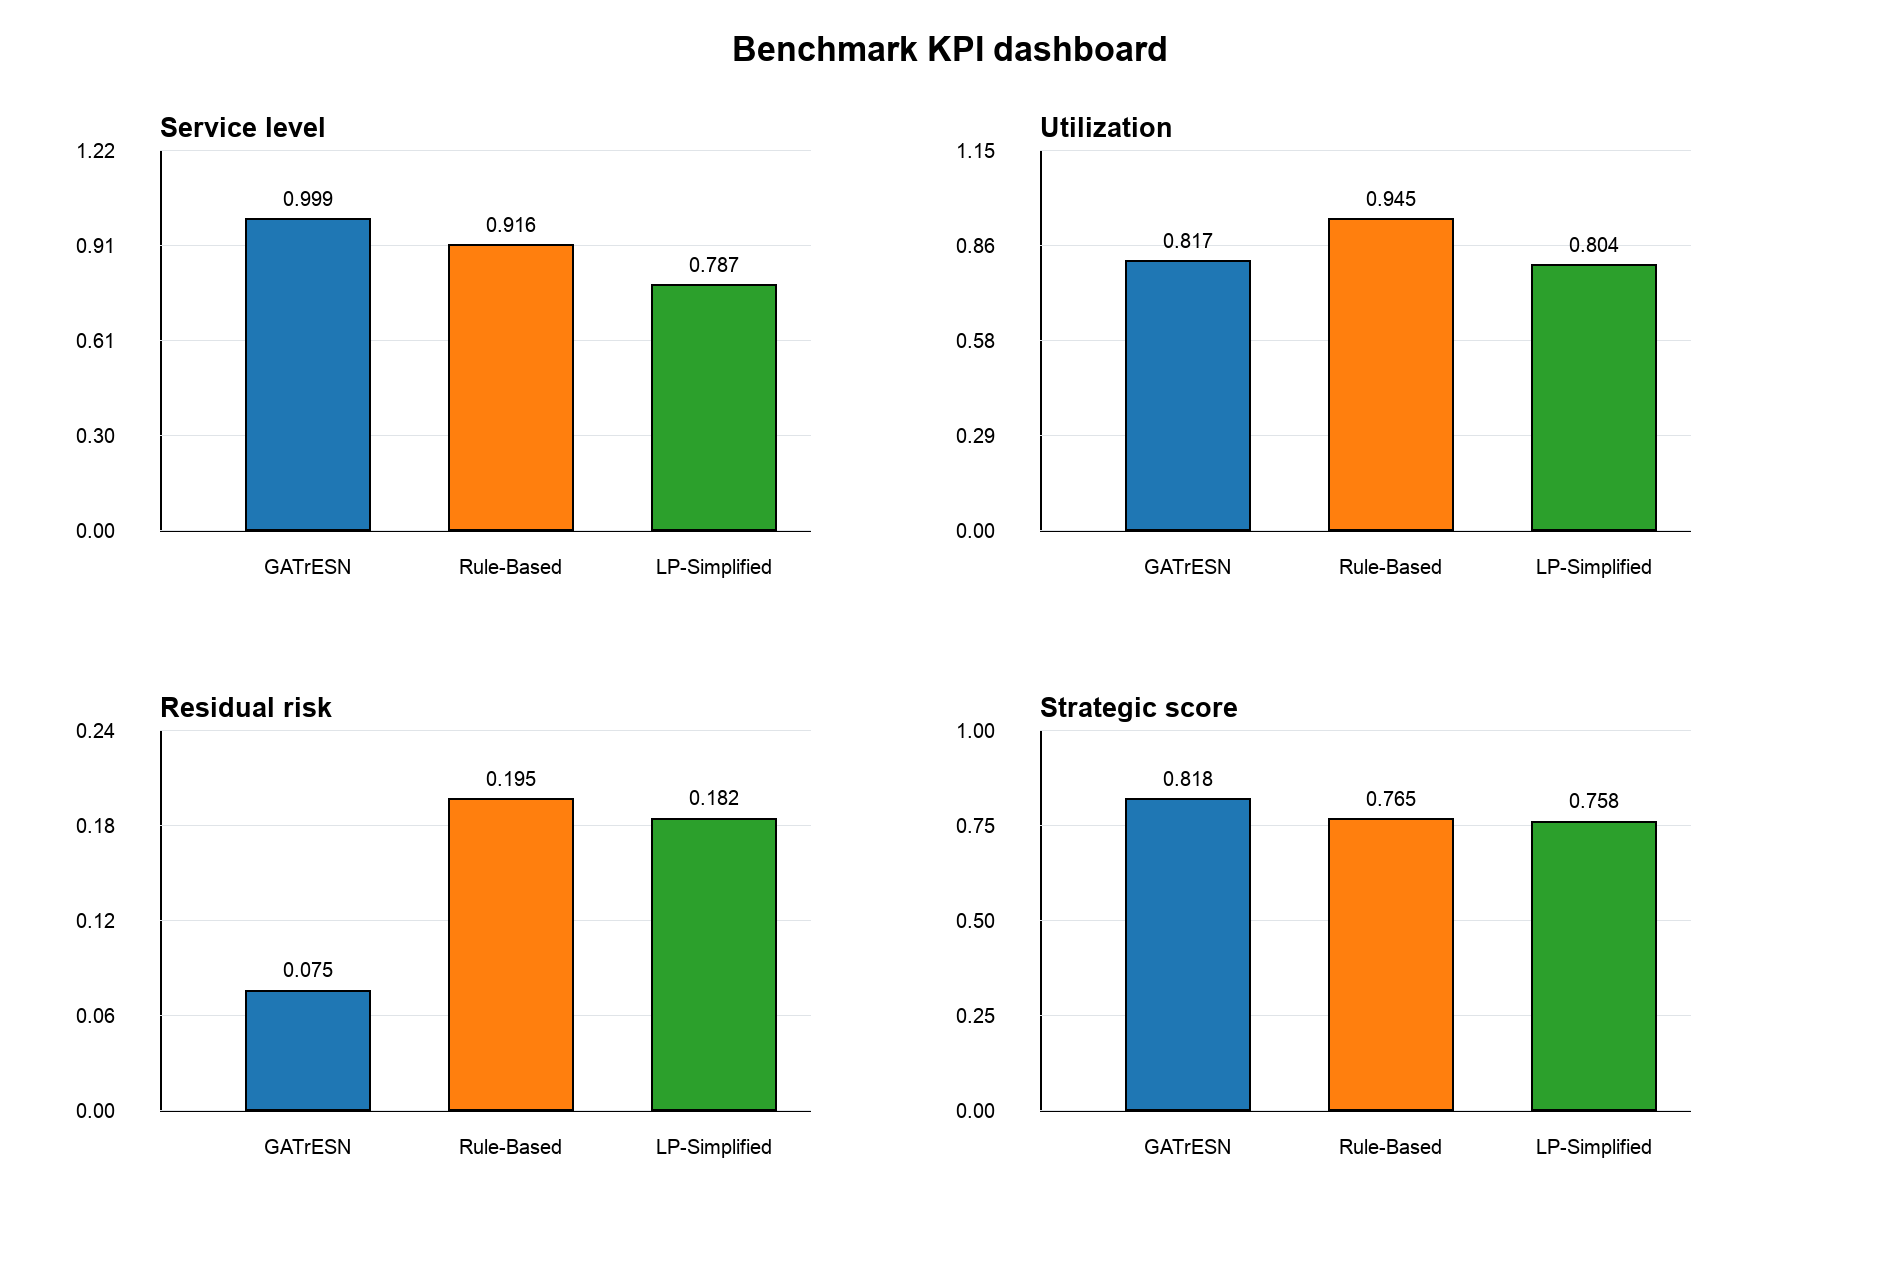
\includegraphics[width=0.98\textwidth]{../figures/GATrESN_benchmark_kpi_dashboard.png}
\caption{Benchmark KPI dashboard comparing GATrESN, Rule-Based, and LP-Simplified policies using the same digital twin performance indicators.\label{fig:benchmark_kpi_dashboard}}
\end{figure}

Figure~\ref{fig:benchmark_kpi_dashboard} summarizes the main KPI trade-offs. GATrESN dominates the two benchmarks in service level, residual risk, and composite strategic score. Rule-Based achieves the highest mean utilization, but this occurs together with higher residual risk and lower service reliability, indicating that high utilization is partly obtained by operating closer to capacity pressure. LP-Simplified achieves the lowest expected cost, as expected from its linear cost-minimization structure, but it produces the lowest service level and does not reduce residual risk as effectively as GATrESN. Therefore, the comparison shows that the proposed method is not merely optimizing a single KPI; it shifts the policy balance toward robustness and service continuity.

\begin{figure}[H]
\centering
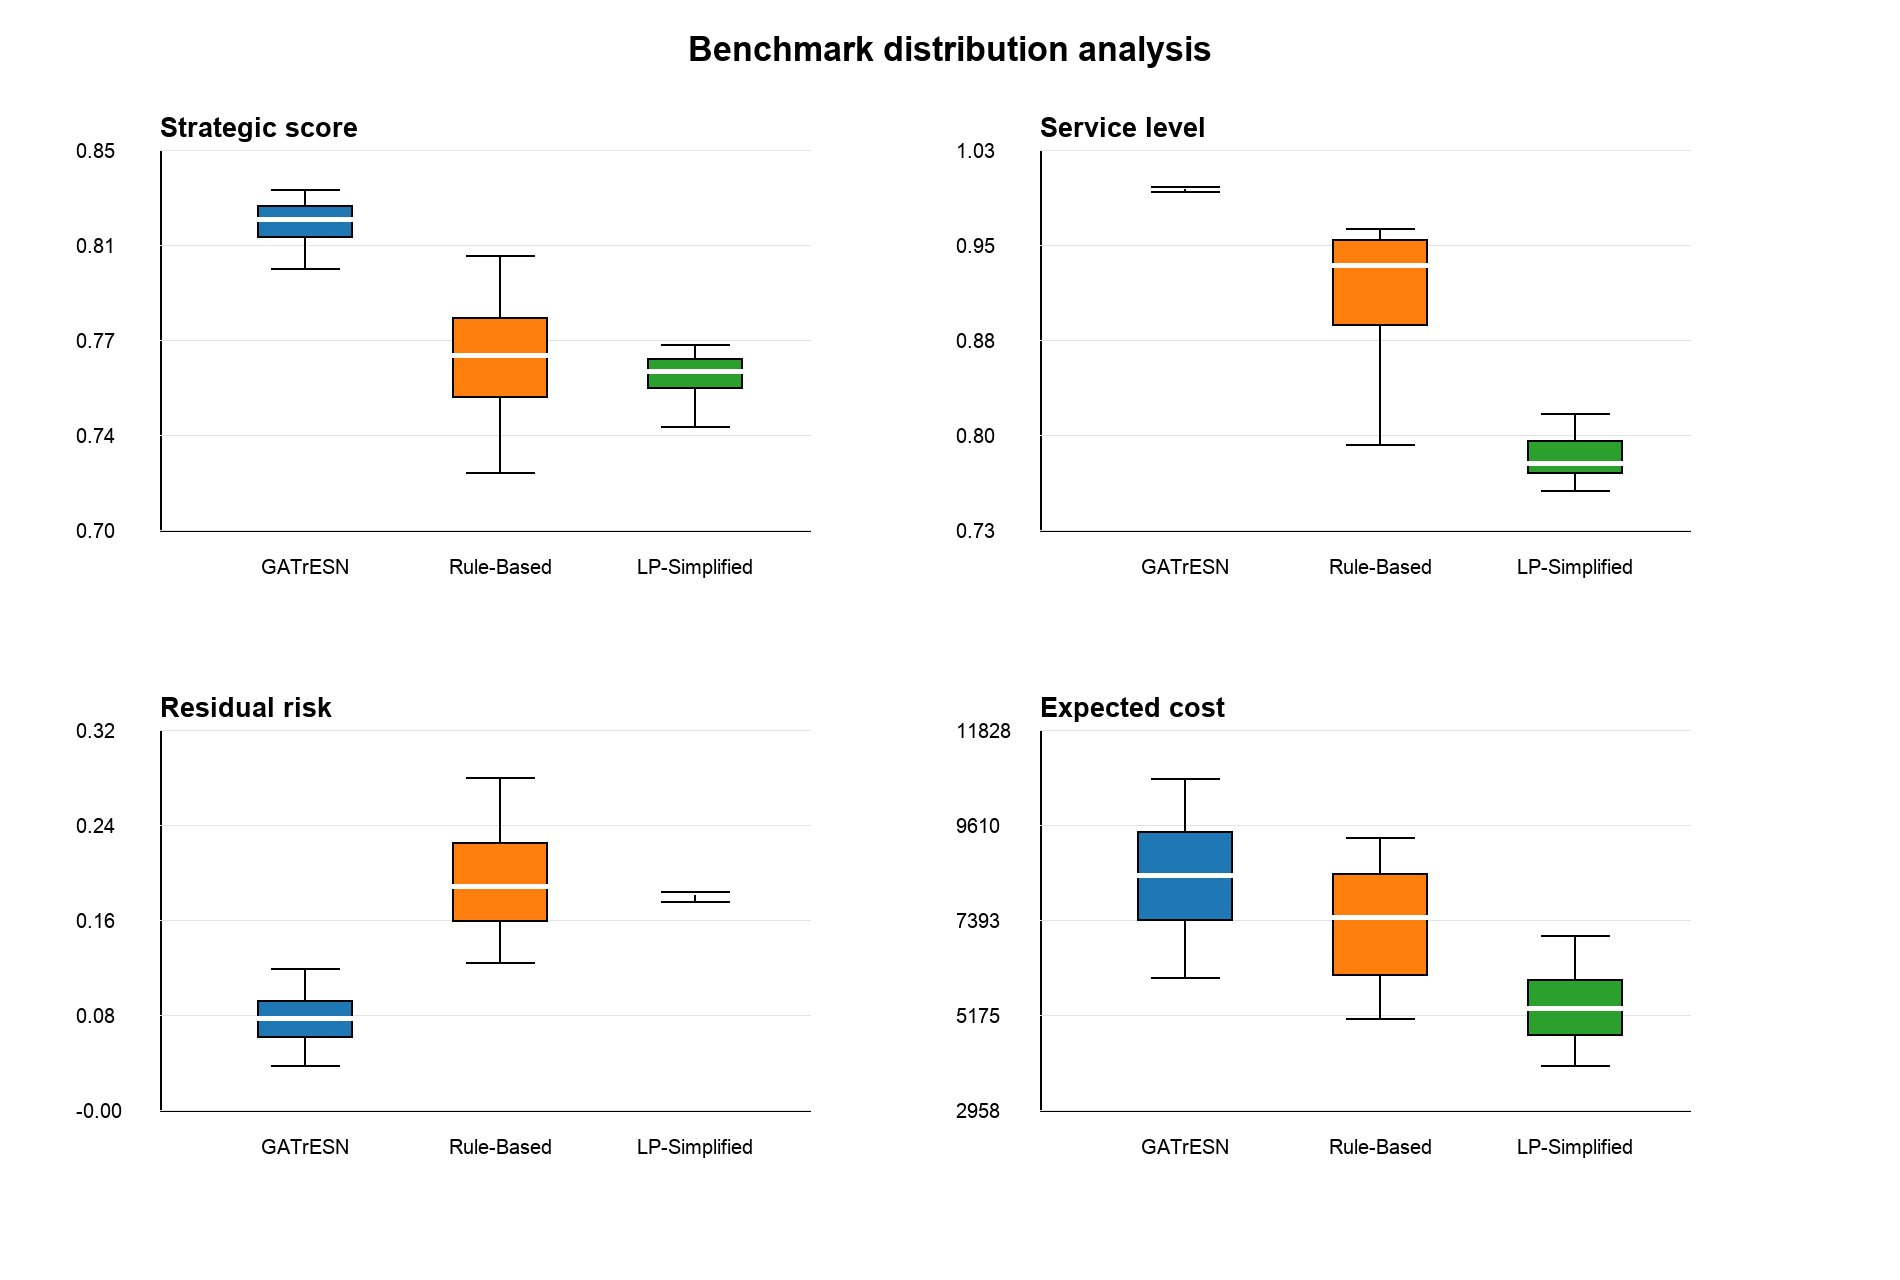
\includegraphics[width=0.98\textwidth]{../figures/GATrESN_benchmark_distribution_analysis.png}
\caption{Distributional benchmark analysis across strategic decision instances. Boxes represent interquartile ranges, median lines, and 5th--95th percentile whiskers for each model.\label{fig:benchmark_distribution_analysis}}
\end{figure}

Figure~\ref{fig:benchmark_distribution_analysis} provides a distributional view of the same comparison. GATrESN shows a narrow strategic-score distribution with a median of 0.819 and a 5th--95th percentile interval of 0.800--0.831. Rule-Based has a lower median strategic score of 0.767 and a wider distribution, while LP-Simplified remains concentrated around a lower score region. The service-level distribution also indicates that GATrESN maintains near-complete fulfillment for most decision instances, whereas Rule-Based exhibits a broader range and LP-Simplified remains capped by the linearized service approximation. In residual risk, GATrESN is concentrated around lower values, with a median of 0.075 and a 95th percentile of 0.118, compared with 0.189 and 0.283 for Rule-Based and 0.184 and 0.185 for LP-Simplified. These results suggest that the proposed model improves not only average performance but also downside behavior.

To validate whether the observed differences persist at the instance level, a paired statistical analysis was performed using the 1800 matched digital twin decision states. For each KPI and benchmark, the paired advantage was computed as GATrESN minus the benchmark for strategic score and service level, and as the benchmark residual risk minus GATrESN residual risk for risk reduction. Therefore, positive values in Table~\ref{tab:statistical_validation} consistently indicate an advantage for GATrESN. The validation used bootstrap 95\% confidence intervals for the mean paired advantage, a two-sided paired sign test, Holm adjustment across the six pairwise tests, and Cohen's $d_z$ as a paired effect-size measure.

\begin{table}[H]
\caption{Paired statistical validation of GATrESN advantages across matched decision instances.\label{tab:statistical_validation}}
\begin{tabularx}{\textwidth}{CCCCCC}
\toprule
\textbf{Metric} & \textbf{Comp.} & \textbf{Mean adv.} & \textbf{95\% CI} & \textbf{Dominance} & \textbf{$d_z$}\\
\midrule
Strategic score & vs. Rule-Based & 0.0525 & [0.0512, 0.0538] & 98.72\% & 1.92\\
Strategic score & vs. LP-Simplified & 0.0594 & [0.0590, 0.0598] & 100.00\% & 6.14\\
Service level & vs. Rule-Based & 0.0835 & [0.0810, 0.0861] & 99.17\% & 1.52\\
Service level & vs. LP-Simplified & 0.2124 & [0.2114, 0.2134] & 100.00\% & 9.95\\
Residual risk reduction & vs. Rule-Based & 0.1199 & [0.1177, 0.1221] & 100.00\% & 2.53\\
Residual risk reduction & vs. LP-Simplified & 0.1075 & [0.1063, 0.1087] & 99.89\% & 4.09\\
\bottomrule
\end{tabularx}
\end{table}

All bootstrap intervals in Table~\ref{tab:statistical_validation} are strictly positive, indicating that the paired mean advantage remains above zero for all evaluated KPIs and benchmark comparisons. The Holm-adjusted sign-test results were significant for all six comparisons ($p < 0.001$), and the paired effect sizes were large in every case. This confirms that the superiority of GATrESN is not driven by a small number of favorable cases or by aggregate averaging alone; it is consistently observed across the matched decision-state distribution generated by the digital twin.

\begin{figure}[H]
\centering
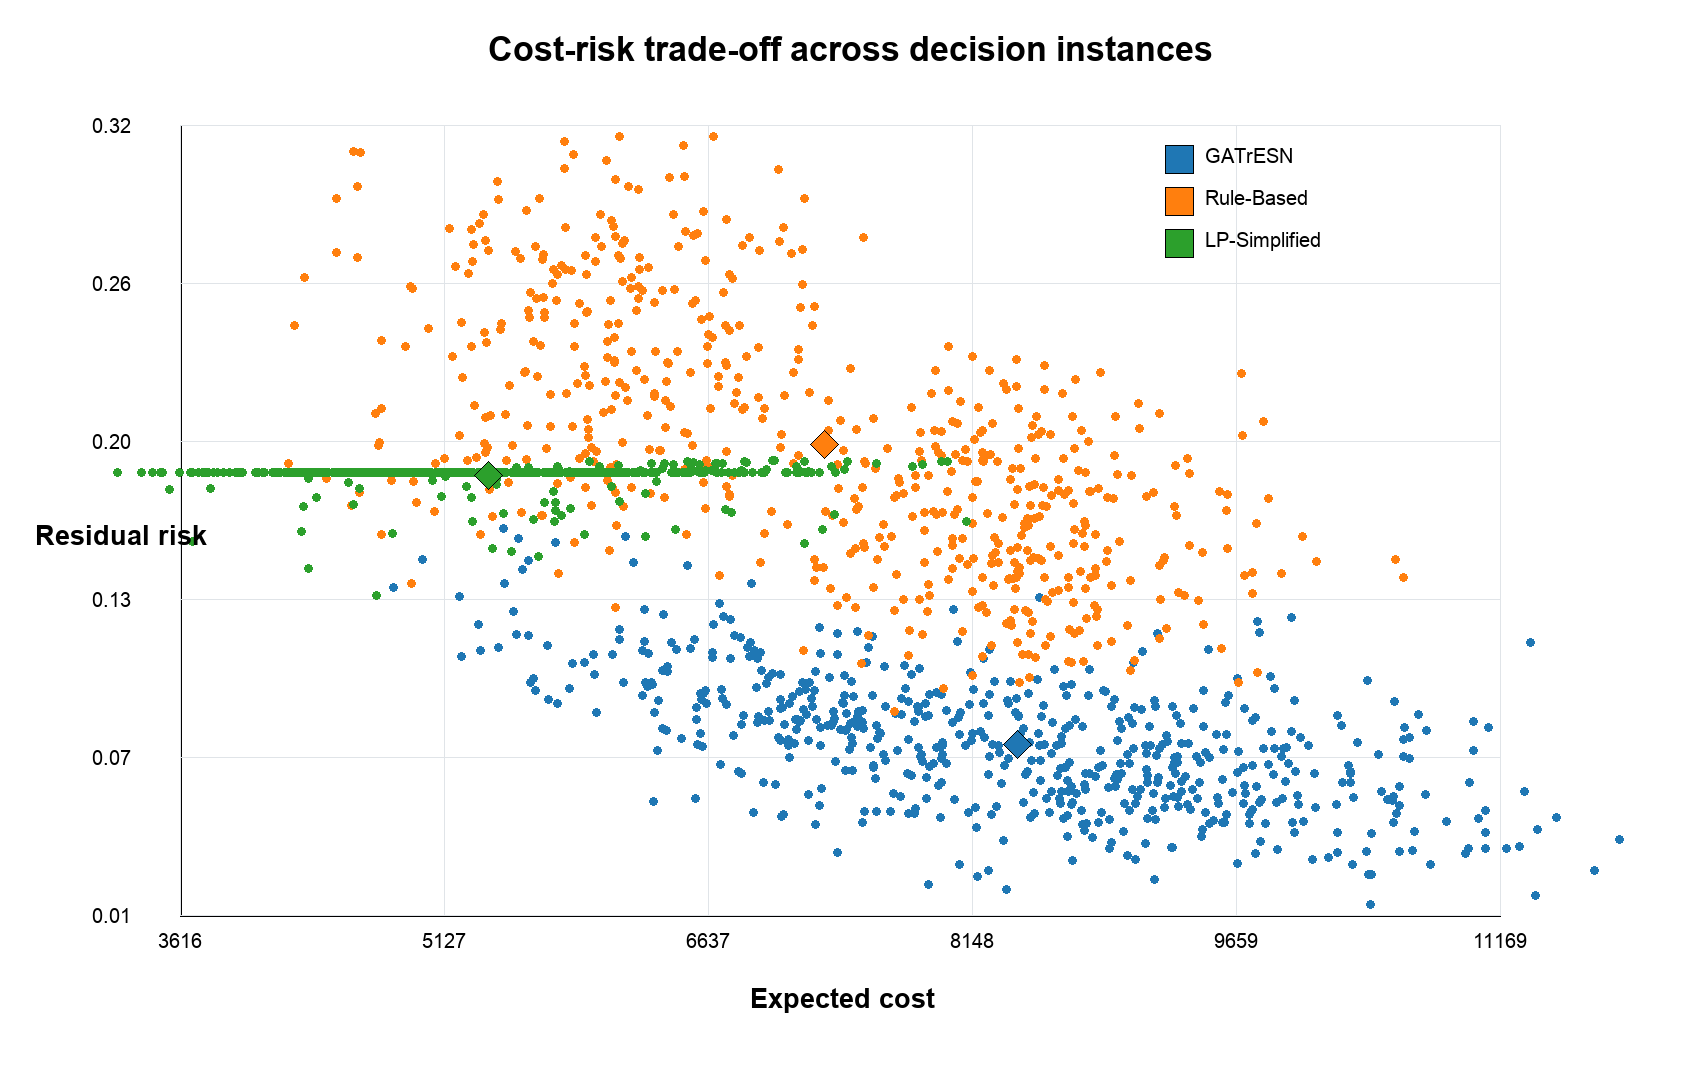
\includegraphics[width=0.98\textwidth]{../figures/GATrESN_cost_risk_tradeoff.png}
\caption{Cost--risk trade-off across matched decision instances. Small points represent sampled decisions, and diamond markers represent model means.\label{fig:cost_risk_tradeoff}}
\end{figure}

Figure~\ref{fig:cost_risk_tradeoff} clarifies why the GATrESN solution differs from the two benchmarks. LP-Simplified occupies the low-cost region but remains at a higher residual-risk band, because its deterministic linear policy prioritizes cost and satisfies only simplified service and risk constraints. Rule-Based occupies a middle-cost region but with substantial risk dispersion, reflecting the discontinuous behavior of threshold policies. GATrESN moves toward higher expected cost but substantially lower residual risk, indicating that the GA selected policy packages that invest in resilience and operational buffers when the digital twin projected risk-sensitive future states. This is consistent with the role of GATrESN as a robust strategic decision model rather than a nominal cost optimizer.

The optimized decision variables also show that the case is not solved by a single trivial policy. Across 1800 decision instances, GATrESN selected a mean capacity multiplier of 1.113, a mean cost-policy multiplier of 0.950, a mean resilience investment of 0.816, a mean inventory buffer of 0.662, a mean workforce-flexibility level of 0.611, and a mean supplier-redundancy level of 0.672. The dispersion across these levers indicates that the GA adapted the policy package to the digital twin state rather than applying one fixed rule to all decision instances. At the instance level, GATrESN produced the highest strategic score in 98.72\% of matched decisions, the highest service level in 99.67\% of decisions, and the lowest residual risk in 99.89\% of decisions. These dominance rates reinforce the conclusion that the proposed ESN--attention--GA coupling creates prescriptive value beyond both deterministic linear optimization and managerial threshold rules.

%%%%%%%%%%%%%%%%%%%%%%%%%%%%%%%%%%%%%%%%%%
\section{Discussion}
The results show that the proposed framework can move the digital twin from a descriptive representation of operations toward a predictive and prescriptive decision environment. The main implication is that the digital twin is not treated as a visualization layer or a passive data repository. Instead, it becomes a structured digital laboratory in which operational states are reconstructed, future demand--risk conditions are projected, candidate policies are stress-tested, and KPI feedback is returned to the virtual representation. This is important for strategic operations management because many managerial decisions must be evaluated before implementation, especially when they involve costly capacity adjustments, resilience investments, inventory buffers, workforce flexibility, or supplier-redundancy commitments.

The benchmark results indicate that the value of GATrESN does not come from optimizing a single KPI in isolation. The proposed model increased service reliability and reduced residual risk while accepting a higher expected cost. This behavior is consistent with a strategic robustness perspective: the model selected policies that invested in operational protection when the digital twin projected risk-sensitive states. LP-Simplified produced lower expected cost, as expected from a deterministic cost-oriented approximation, but it remained exposed to higher residual risk and lower service performance. Rule-Based achieved high utilization, but with greater risk dispersion and weaker strategic-score performance. Therefore, the trade-off observed in the results should be interpreted as a strategic cost--resilience reallocation rather than as a simple cost inefficiency.

The paired statistical validation strengthens this interpretation. Because GATrESN and the two benchmark policies were evaluated on the same 1800 digital twin decision states, the comparison controls for the underlying demand, risk, capacity, and cost conditions. The bootstrap intervals, dominance rates, Holm-adjusted sign tests, and paired effect sizes show that the observed gains are not driven by isolated favorable cases. Instead, the advantage appears consistently across the matched state distribution. This supports the argument that the ESN--attention--GA coupling provides prescriptive value beyond both deterministic linear planning and threshold-based managerial heuristics.

From a methodological perspective, the hybrid structure of GATrESN is central. The ESN provides nonlinear temporal memory without requiring full recurrent-network training, which supports reproducibility and computational efficiency. The attention layer allows the model to weight historical states according to their relevance for the current forecast, which is important when disruption effects persist over time. The GA then searches the bounded nonlinear policy space under scenario uncertainty. Embedding these components inside the same digital twin prevents the common separation between forecasting, simulation, and optimization. Forecasts are not reported as an end product; they are used to generate scenarios and prescribe decisions. Similarly, optimization is not performed on a static deterministic input; it is conditioned on a learned virtual state and evaluated through KPI feedback.

The study also has limitations. The operational data structure and disruption dynamics are controlled by the computational case-study design, which allows reproducibility but does not capture all organizational, behavioral, and institutional constraints of a specific enterprise. The benchmark LP model is intentionally simplified to represent deterministic analytical planning; more advanced stochastic, robust, or mixed-integer formulations could be added in future comparisons. Likewise, the current attention layer is used as a temporal weighting mechanism rather than as a fully trained deep Transformer architecture. Future work may extend the framework using real-time enterprise-system integration, richer uncertainty models, explainable policy diagnostics, multi-objective Pareto analysis, and additional benchmark families such as robust optimization, reinforcement learning, and model predictive control.

%%%%%%%%%%%%%%%%%%%%%%%%%%%%%%%%%%%%%%%%%%
\section{Conclusions}
This study presented GATrESN, an AI-driven digital twin framework for strategic operations management. The framework integrates digital twin state representation, Echo State Networks, Transformer-style attention, Genetic Algorithms, Monte Carlo scenario simulation, KPI feedback, and multi-criteria decision support. The proposed approach treats the organization as a dynamic virtual twin rather than as a static optimization problem, allowing strategic decisions to be evaluated under plausible future conditions before managerial implementation.

The case study was organized as a longitudinal site--product--period operational panel and transformed into lagged digital twin states for predictive--prescriptive modeling. Across 1800 matched decision instances, GATrESN achieved the highest mean strategic score, the highest service-level performance, and the lowest residual risk relative to LP-Simplified and Rule-Based benchmarks. The paired statistical validation confirmed that these advantages were consistent across decision states, with positive bootstrap confidence intervals, high dominance rates, significant Holm-adjusted sign-test results, and large paired effect sizes. These findings indicate that the proposed model improves not only average benchmark performance but also the reliability of decisions across heterogeneous operational conditions.

The main contribution of the paper is the integration of temporal learning, attention-based dependency extraction, scenario simulation, and evolutionary prescriptive optimization inside a reproducible digital twin workflow. In practical terms, GATrESN provides a digital laboratory for testing strategic policies before implementation, quantifying service--cost--risk trade-offs, and supporting adaptive managerial learning through KPI feedback. Future research may extend the framework using empirical organizational data, real-time enterprise systems, richer benchmark models, explainable AI methods, and multi-objective decision interfaces for strategic operations management.

%%%%%%%%%%%%%%%%%%%%%%%%%%%%%%%%%%%%%%%%%%
\authorcontributions{Conceptualization, C.H.V. and L.M.V.; methodology, C.H.V.; software, C.H.V.; validation, C.H.V. and L.M.V.; formal analysis, C.H.V.; investigation, C.H.V. and L.M.V.; data curation, C.H.V.; writing---original draft preparation, C.H.V.; writing---review and editing, C.H.V. and L.M.V.; visualization, C.H.V.; supervision, L.M.V. All authors have read and agreed to the published version of the manuscript.}

\funding{This research received no external funding.}

\institutionalreview{Not applicable.}

\informedconsent{Not applicable.}

\dataavailability{The data used in this study are synthetically generated for methodological demonstration and reproducibility purposes. The MATLAB code used to generate the dataset and reproduce the simulation results is provided with the manuscript materials.}

\acknowledgments{The authors acknowledge the use of computational tools for simulation, numerical analysis, and manuscript preparation.}

\conflictsofinterest{The authors declare no conflicts of interest.}

%%%%%%%%%%%%%%%%%%%%%%%%%%%%%%%%%%%%%%%%%%
\reftitle{References}
\bibliography{../references/references}

\end{document}
